\subsection{Example}

\begin{code}[js,
  caption={Example web application},
  label={lst:source}]
var app = require('express')(),
    fs = require('fs'),
    count = 0; //@\label{lst:source-counter}@

app.get('/', function handler(req, res){ //@\label{lst:source-handler}@
  fs.readFile(__filename, function reply(err, data) {
    count += 1;
    res.send(err || template(count, data)); //@\label{lst:source-send}@
  });
}); //@\label{lst:source-handler-end}@

app.listen(8080);
\end{code}

\begin{figure}[h!]
  \centering
  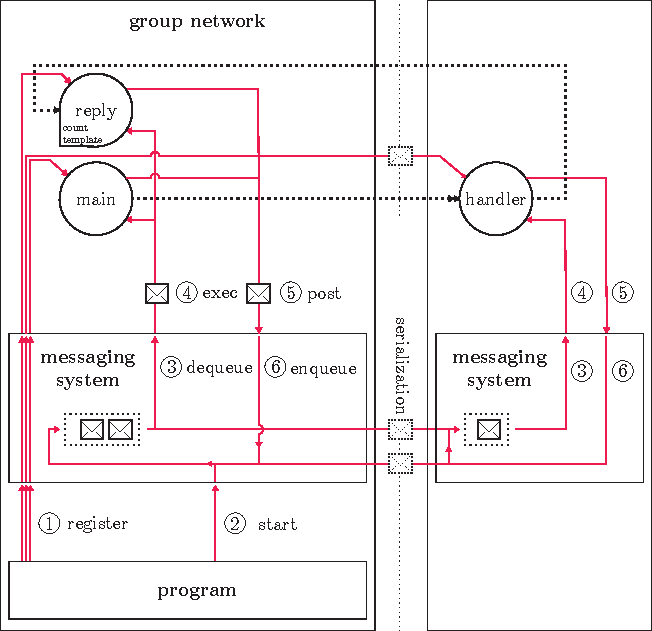
\includegraphics[width=0.7\linewidth]{../resources/schema-message.pdf}
  \caption{The fluxional execution model in details}
  \label{fig:MesSys}
\end{figure}

% \begin{wrapfigure}{r}{0.60\textwidth}
%   \vspace{-25pt}
%   \begin{center}
%     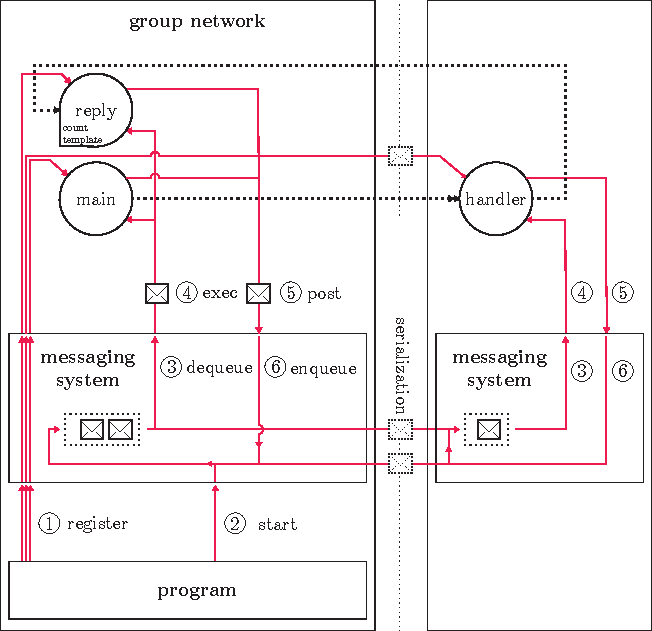
\includegraphics[width=\linewidth]{../resources/schema-message.pdf}
%     \caption{The fluxional execution model in details}
%     \label{fig:MesSys}
%   \end{center}
%   \vspace{-10pt}
% \end{wrapfigure}

% The fluxional execution model is illustrated with an example application presented in listing \ref{lst:source}.
The example application in listing \ref{lst:source} reads a file, and sends it back along with a request counter.
The \texttt{handler} function, line \ref{lst:source-handler} to \ref{lst:source-handler-end}, receives the input stream of requests.
The \texttt{count} variable at line \ref{lst:source-counter} counts the requests, and needs to be saved between two messages receptions.
The \texttt{template} function formats the output stream to be sent back to the client.
The \texttt{app.get} and \texttt{res.send} functions, lines \ref{lst:source-handler} and \ref{lst:source-send}, interface the application with the clients.
Between these two interface functions is a chain of three functions to process the client requests : \texttt{app.get} $\to$ \hspace{-1.4em} $\to$ \texttt{handler} $\to$ \texttt{reply}.
This chain of functions is transformed into a pipeline, expressed in the high-level fluxional language in listing \ref{lst:fluxional}.
The transformation process between the source and the fluxional code is explained in \ref{chapter5}, in section \ref{chapter5:flx:compiler}.

The execution is illustrated in figure \ref{fig:MesSys}.
The dashed arrows between fluxions represent the message streams as seen in the fluxional application.
The plain arrows represent the operations of the messaging system during the execution.
These steps are indicated by numeroted circles.
The \textit{program} registers its fluxions in the messageing system, \circled{1}.
The fluxion \textit{reply} has a context containing the variable \texttt{count} and \texttt{tem\-plate}.
When the application receives a request, the first fluxion in the stream, \textit{main}, queues a \texttt{start} message containing the request, \circled{2}.
This first message is to be received by the next fluxion \textit{handler}, \circled{3}, and triggers its execution, \circled{4}.
The fluxion \textit{handler} sends back a message, \circled{5}, to be enqueued, \circled{6}.
The system loops through steps \circled{3} through \circled{6} until the queue is empty.
This cycle starts again for each new incoming request causing another \texttt{start} message.

\begin{code}[flx, caption={Example application expressed in the high-level fluxional language}, label={lst:fluxional}]
flx main & grp_res
>> handler [res]
  var app = require('express')(),
      fs = require('fs'),
      count = 0;

  app.get('/', >> handler); //@\label{lst:fluxional-streamtohandler}@
  app.listen(8080);

flx handler
-> reply [res]
  function handler(req, res) {
    fs.readFile(__filename, -> reply); //@\label{lst:fluxional-readfile}@
  }

flx reply & grp_res {count, template}
-> null
  function reply(error, data) {
    count += 1; //@\label{lst:fluxional-counter}@
    res.send(err || template(count, data)); //@\label{lst:fluxional-ressend}@
  }
\end{code}

The chain of functions from listing \ref{lst:source} is expressed in the fluxional language in listing \ref{lst:fluxional}.
The fluxion \texttt{handler} doesn't have any dependencies, so it can be executed in a parallel event-loop.
The fluxions \texttt{main} and \texttt{reply} belong to the group \texttt{grp\_res}, indicating their dependency over the variable \texttt{res}.
The group name is chosen arbitrarily.
All the fluxions inside a group are executed sequentially on the same event-loop, to protect the shared variables against concurrent accesses.

The variable \texttt{res} is created and consumed within a chain of \textit{post} stream.
Therefore, it is exclusive to one request and cannot be propagated to another request.
It doesn't prevent the whole group from being replicated.
However, the fluxion \texttt{reply} depends on the variable \texttt{count} created upstream the \textit{start} stream, which prevents this replication.
If it did not rely on this state, the group \texttt{grp\_res} would be stateless, and could be replicated to cope with the incoming traffic.

\separator

This execution model allows to parallelize the execution of an application as a pipeline, as with the fluxion \texttt{handler}.
And some parts are replicated, as could be the group \texttt{grp\_res}.
This parallelization improves the efficiency of the application.
Indeed, as a fluxion contains its state and expresses its dependencies, it can be migrated.
It allows to adapt the number of fluxions per core to adjust the resource usage in function of the desired throughput.

Yet, the parallelization is limited by the dependencies between fluxions.
A developer can ignore these dependencies at first, to focus on productivity.
And then continuously tune the implementation to remove these dependencies and improve efficiency.
This continuous tuning avoid the disruptive shifts of technology required by current platforms.